%!TEX program = xelatex
\documentclass[12pt]{article}
\usepackage[top=1.5cm, left=2cm, right=2cm, bottom=1.5cm]{geometry} % Symmetrical margins
\usepackage{graphicx}
\usepackage{amsmath}
\usepackage{fontspec}
\usepackage{polyglossia}
% \usepackage[polutonikogreek,english]{hyphenat}
\usepackage{xunicode}
\usepackage{xltxtra}
\usepackage{float}
\usepackage{placeins}
\usepackage{indentfirst}
\usepackage{nicefrac}
\usepackage{booktabs}
\usepackage{array}
\usepackage{xcolor}
\usepackage{minted}
\usepackage{varwidth}

\usepackage{pgfplotstable}
\usepackage{subcaption}

\usepackage[
    backend=biber,
    sorting=nyt
]{biblatex}
\addbibresource{references.bib}
\DefineBibliographyStrings{greek}{
    andothers = {κ.α}
}
\DeclareFieldFormat*{title}{\textnormal{#1}}
%\usepackage[utf8]{inputenc}
%\usepackage[greek,english]{babel}
\setdefaultlanguage[variant=monotonic]{greek}
\setotherlanguage{english}

\usepackage[colorlinks=true,
            linkcolor=black,
            urlcolor=blue,
            citecolor=blue]{hyperref}

\setmainfont[Scale=1.09]{DejaVuSans}
\newfontfamily\greekfont[Scale=1.09]{FreeSerif}
\newfontfamily\greekfontsf[Scale=1.09]{FreeSans}
\newfontfamily\greekfonttt[Scale=1.09]{FreeMono}
\setromanfont{FreeSerif}
\setsansfont{FreeSans}
\setmonofont{FreeMono}

\setminted{fontsize=\small}
\usemintedstyle{perldoc}
% \definecolor{monokai}{RGB}{39,40,34}
\definecolor{paraiso-light}{RGB}{231, 233, 219}


\usepackage{titlesec}

\titleformat{\section}
    {\normalfont\Large\bfseries}
    {\thesection}
    {1.5em}
    {\vspace{1em}}
%\setlength{\droptitle}{-3cm}

\begin{document}

\title{Crimmins Speckle Removal Filter}
\author{Αναστάσιος Φραγκόπουλος 58633}
\date{}


\begin{titlepage}
    \begin{center}
        \vspace*{1.5cm}

        \textbf{\LARGE Crimmins Speckle Removal Filter}

        \vspace{0.5cm}
        {\large Τεχνολογία Παράλληλης Επεξεργασίας}

        \vspace{1.5cm}

        \textbf{Αναστάσιος Φραγκόπουλος 58633}

        \vfill

        Πρώτη εξαμηνιαία εργασία

        Ακαδ. Έτος 2024-2025

        \vspace{0.8cm}

        Εργαστήριο Αρχιτεκτονικής Υπολογιστών και Συστημάτων Υψηλών Επιδόσεων\\
        Δημοκρίτειο Πανεπιστήμιο Θράκης\\
        Τμήμα Ηλεκτρολόγων Μηχανικών και Μηχανικών Υπολογιστών\\

    \end{center}
\end{titlepage}


\tableofcontents
\newpage


\section{Σειριακός Αλγόριθμος}

Ο Crimmins Speckle removal είναι ένας αλγόριθμος που μειώνει από ασπρόμαυρες εικόνες τον θόρυβο salt-and-pepper, που είναι ένα είδος θορύβου που δίνει την εμφάνιση μίας εικόνας πασπαλισμένης με αλάτι και πιπέρι. Οι επανειλημμένες χρήσεις του αλγόριθμου σε μια εικόνα δίνουν καλύτερα αποτελέσματα μείωσης του θορύβου αλλά προκαλούν θόλωση της εικόνας.

Ο αλγόριθμος αρχικά αυξάνει την φωτεινότητα των pixel που είναι σκοτεινότερα από τους γείτονες του και μετά μειώνοντας την φωτεινότητα των pixel που είναι φωτεινότερα από τους γείτονες του. Η σύγκρηση αυτή γίνεται μεταξύ του κάθε pixel και ζευγαριού pixel των 8 γειτόνων για μια κατεύθυνση σε κάθε πέρασμα (πάνω-κάτω, δεξιά-αριστερά, διαγώνια αριστερά-δεξιά, διαγώνια δεξιά-αριστερά).

Για κάθε επανάληψη του αλγορίθμου, γίνονται πρώτα οι παρακάτω συγκρίσεις για την διόρθωσή των σκοτεινών pixel για τις τέσσερεις κατευθύνσεις

\begin{minted}[breaklines, breaksymbolright={}, breaksymbolleft={}, bgcolor=paraiso-light]{c}
    uint8_t dark_pass_logic(uint8_t a, uint8_t b, uint8_t c)
    {
            if(a >= b + 2) b++;
            if(a > b && b <= c) b++;
            if(c > b && b <= a) b++;
            if(c >= b + 2) b++;
            return b;
    }
\end{minted}

και έπειτα οι παρακάτω συγκρίσεις για την διόρθωση των φωτεινών pixel για τις τέσσερεις κατευθύνσεις

\begin{minted}[breaklines, breaksymbolright={}, breaksymbolleft={}, bgcolor=paraiso-light]{c}
    uint8_t light_pass_logic(uint8_t a, uint8_t b, uint8_t c)
    {
            if(a <= b - 2) b--;
            if(a < b && b >= c) b--;
            if(c < b && b >= a) b--;
            if(c <= b - 2) b--;
            return b;
    }
\end{minted}

Όπου b το κεντρικό pixel κάθε γειτονιάς και a, c το ζευγάρι pixel για μια κατεύθυνσή (π.χ. για την επανάληψη πάνω-κάτω το a θα είναι το pixel πάνω από το b και το c το pixel κάτω από το b).\\

Οπότε για μία επανάληψη του, ο αλγόριθμος περνάει όλα τα pixel μίας εικόνας τέσσερις φορές για την διόρθωση των σκοτεινών και άλλες τέσσερεις για την διόρθωση των φωτεινών pixel. Δηλαδή κάνει $8\cdot m \cdot n$ επαναλήψεις όπου m το πλάτος και n το μήκος της εικόνας σε pixel. Άρα η πολυπλοκότητα του είναι  $\mathrm{O}(k \cdot m \cdot n)$, όπου k είναι ο αριθμός των επαναλήψεων του αλγόριθμου για μια εικόνα.

\begin{figure}[H]
    \centering
    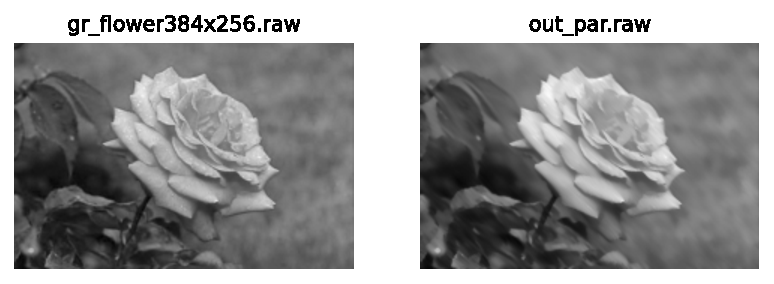
\includegraphics[width=0.8\linewidth]{./pics/gr_flower384x256.pdf}
    \caption{Παράδειγμα αλγορίθμου για 2 επαναλήψεις}
\end{figure}

\begin{figure}[H]
    \centering
    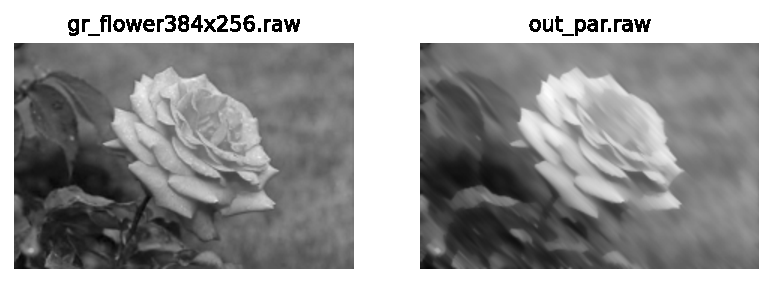
\includegraphics[width=0.8\linewidth]{./pics/gr_flower384x256_blur.pdf}
    \caption{Παράδειγμα αλγορίθμου για 8 επαναλήψεις}
\end{figure}

\vspace{2em}

\section{Υλοποίηση του αλγόριθμου}

Κύριο στοιχείο στην υλοποίηση του αλγόριθμου είναι η συνάρτηση που είναι υπεύθυνη για το πέρασμα του κάθε pixel της εικόνας και είναι φτιαγμένη έτσι ώστε να μπορεί να ξαναχρησιμοποιηθεί για όλες τις κατευθύνσεις ανάλογα με την είσοδο που της δίνεται. Επιπλέον, οι συναρτήσεις που κάνουν την σύγκρισή των γειτονικών pixel, που αναφέρθηκαν παραπάνω δίνονται ως είσοδος στην συνάρτηση για τον ίδιο λόγο. Η κάθε επανάληψη της εξωτερικής for loop μεταβάλει την γραμμή της εικόνας στην οποία βρισκόμαστε και η εσωτερική μεταβάλει την στήλη της εικόνας στην οποία βρισκόμαστε. Στην αλλαγή γραμμής υπολογίζουμε έναν pointer που δείχνει στην αρχή κάθε γραμμής, για το a, b, c, ώστε να γλιτώσουμε ένα μέρος των πράξεων που χρειάζεται στις επαναλήψεις του άξονα x. Τέλος, γράφει στο pixel b την τιμή διασφαλίζοντας ότι θα είναι μεταξύ 0 και 255.

\newpage

\begin{minted}[breaklines, breaksymbolright={}, breaksymbolleft={}, bgcolor=paraiso-light]{c}
void pass_func(uint8_t *image, uint8_t *tmp_image, uint32_t width,
    uint32_t height, int dx, int dy,
    uint8_t (*pass_logic_func)(uint8_t, uint8_t, uint8_t)) {

    for(int y = 1; y < height - 1; y++) {
        uint8_t *row_a = tmp_image + (y-dy) * width;
        uint8_t *row_b = tmp_image + y * width;
        uint8_t *row_c = tmp_image + (y+dy) * width;
        uint8_t *row_out = image + y * width;

        for(int x = 1; x < width - 1; x++) {
            uint8_t a = row_a[x-dx];
            uint8_t b = row_b[x];
            uint8_t c = row_c[x+dx];

            b = pass_logic_func(a, b, c);
            row_out[x] = (b < 0) ? 0 : (b > 255) ? 255 : b;
        }
    }
}
\end{minted}

Οι πράξεις για την επιλογή των a, b, c φαίνεται από το παρακάτω διάγραμμα που δείχνει τις συντεταγμένες (x, y) του κάθε pixel μίας γειτονιάς.

\vspace{0.3em}
\begin{center}
\begin{varwidth}{0.6\linewidth}
\begin{minted}[breaklines, breaksymbolright={}, breaksymbolleft={}, bgcolor=paraiso-light]{sh}
 +------------+------------+------------+ 
 |            |            |            | 
 |  y-1, x-1  |   y-1, x   |  y-1, x+1  | 
 |            |            |            | 
 +------------+------------+------------+ 
 |            |            |            | 
 |  y,   x-1  |   y,   x   |  y,   x+1  | 
 |            |            |            | 
 +------------+------------+------------+ 
 |            |            |            | 
 |  y+1, x-1  |   y+1, x   |  y+1, x+1  | 
 |            |            |            | 
 +------------+------------+------------+ 
\end{minted}
\end{varwidth}
\end{center}

Όπως φαίνεται από την συνάρτηση για κάθε μία από τις 8 επανάληψης της πρέπει να της δίνουμε δύο εικόνες, μία με την προηγούμενη κατάσταση της εικόνας και μία στην οποία θα γράψουμε το αποτέλεσμα. Για να αποφύγουμε την συνεχείς δημιουργία και διαγραφή των buffer μεταξύ των επαναλήψεων, επέλεξα να ανταλλάσω τους pointer των εικόνων, έτσι ώστε η εικόνα στην οποία γράφεται το αποτέλεσμα στην επόμενη επανάληψη να γίνεται η προηγούμενη κατάσταση και η προηγούμενη κατάσταση να γίνεται το καινούργιο αποτέλεσμα.

\newpage


\section{Παράλληλη υλοποίηση του Αλγόριθμου}

Στον Crimmins Speckle removal αλγόριθμο το μόνο που πρέπει να παραμένει σειριακό είναι η σειρά με την οποία κάνουμε τα περάσματα για την διόρθωση των pixel για κάθε κατεύθυνση. Για τον λόγο αυτό επέλεξα να παραλληλοποιήσω την συνάρτηση που είναι υπεύθυνη για αυτά τα περάσματα. Έκανα την εξωτερική for loop παράλληλη έτσι ώστε να χωριστεί η εικόνα σε $\nicefrac{\Large n}{\Large p}$ κομμάτια όπου n οι γραμμές της εικόνας και p οι πυρήνες του συστήματος.

\begin{minted}[breaklines, breaksymbolright={}, breaksymbolleft={}, bgcolor=paraiso-light]{c}
void pass_func_par(uint8_t *image, uint8_t *tmp_image, uint32_t width,
    uint32_t height, int dx, int dy,
    uint8_t (*pass_logic_func)(uint8_t, uint8_t, uint8_t), int chunk)
{
    #pragma omp parallel for schedule(static, chunk)
    for(int y = 1; y < height - 1; y++) {
        uint8_t *row_a = tmp_image + (y-dy) * width;
        uint8_t *row_b = tmp_image + y * width;
        uint8_t *row_c = tmp_image + (y+dy) * width;
        uint8_t *row_out = image + y * width;

        for(int x = 1; x < width - 1; x++) {
            uint8_t a = row_a[x-dx];
            uint8_t b = row_b[x];
            uint8_t c = row_c[x+dx];

            b = pass_logic_func(a, b, c);

            row_out[x] = (b < 0) ? 0 :
                (b > 255) ? 255 :
                 b;
        }
    }
}
\end{minted}

Σημαντικό εδώ είναι οτί για τον pxeon2, πριν το τρέξουμε τον παράλληλο αλγόριθμο, πρέπει να θέσουμε τις μεταβλητές συστήματος \verb|OMP_PLACE=cores|, \verb|OMP_PROC_BIND=close|. Ο pxeon2 έχει τέσσερις φυσικούς Intel Xeon Gold 5218 επεξεργαστές ο κάθε ένας με την δικιά του μνήμη και δικιά του cache. Η μεταβλητές αυτές απλά λένε στο openmp να αρχίζει να γεμίζει πρώτα τα threads του ίδιου επεξεργαστή και να μην τα διανέμει ομοιόμορφα σε όλους. Αυτό μας διασφαλίζει ότι τα δεδομένα που χρειάζεται κάθε thread είναι κοντά τους οπότε δεν έχουμε μείωση του χρόνου γιατί πρέπει να επικοινωνήσουν διαφορετικοί επεξεργαστές μεταξύ τους όλη την ώρα. \cite{klemm2023advanced}, \cite{vanderpas2021numa}\\

Για να μπορώ να ελέγξω ότι τα αποτελέσματα του σειριακού και του παράλληλου αλγόριθμου είναι ίδια, έφτιαξα μια συνάρτηση (\verb|image_validator|) που περνάει τις δύο εικόνες και τις ελέγχει pixel προς pixel αν είναι ίδιες.

\newpage
\section{Πειραματικά αποτελέσματα OpenMP}

\begin{table}[htbp]
    \centering
    \begin{subtable}[t]{0.48\textwidth}
        \centering
        \pgfplotstabletypeset[
        col sep=tab,
        header=true,
        columns={threads,{lena256.raw/1 (serial)},{lena256.raw/1 (parallel)},{lena256.raw/1 (speedup)}},
        columns/threads/.style={column name=CPUs},
        columns/{lena256.raw/1 (serial)}/.style={column name=Ts,fixed,precision=4},
        columns/{lena256.raw/1 (parallel)}/.style={column name=Tp,fixed,precision=4},
        columns/{lena256.raw/1 (speedup)}/.style={column name=Sp,fixed,precision=2},
        column type=c,
        every first column/.style={column type=|c},
        column type/.add={|}{|},
        every head row/.style={
            before row=\hline,
            after row=\hline
        },
        every row/.style={
            before row=\hline
        },
        every last row/.style={
            after row=\hline
        }
        ]{./data/result_f1.csv}
        \caption{lena256.raw with 1 iteration}
    \end{subtable}%
    \hfill
    \begin{subtable}[t]{0.48\textwidth}
        \centering
        \pgfplotstabletypeset[
        col sep=tab,
        header=true,
        columns={threads,{mountain1024.raw/1 (serial)},{mountain1024.raw/1 (parallel)},{mountain1024.raw/1 (speedup)}},
        columns/threads/.style={column name=CPUs},
        columns/{mountain1024.raw/1 (serial)}/.style={column name=Ts,fixed,precision=4},
        columns/{mountain1024.raw/1 (parallel)}/.style={column name=Tp,fixed,precision=4},
        columns/{mountain1024.raw/1 (speedup)}/.style={column name=Sp,fixed,precision=2},
        column type=c,
        every first column/.style={column type=|c},
        column type/.add={|}{|},
        every head row/.style={
            before row=\hline,
            after row=\hline
        },
        every row/.style={
            before row=\hline
        },
        every last row/.style={
            after row=\hline
        }
        ]{./data/result_f1.csv}
        \caption{mountain1024.raw with 1 iteration}
    \end{subtable}

    \vspace{8pt}

    \begin{subtable}[t]{0.48\textwidth}
        \centering
        \pgfplotstabletypeset[
        col sep=tab,
        header=true,
        columns={threads,{mountain4096.raw/1 (serial)},{mountain4096.raw/1 (parallel)},{mountain4096.raw/1 (speedup)}},
        columns/threads/.style={column name=CPUs},
        columns/{mountain4096.raw/1 (serial)}/.style={column name=Ts,fixed,precision=4},
        columns/{mountain4096.raw/1 (parallel)}/.style={column name=Tp,fixed,precision=4},
        columns/{mountain4096.raw/1 (speedup)}/.style={column name=Sp,fixed,precision=2},
        column type=c,
        every first column/.style={column type=|c},
        column type/.add={|}{|},
        every head row/.style={
            before row=\hline,
            after row=\hline
        },
        every row/.style={
            before row=\hline
        },
        every last row/.style={
            after row=\hline
        }
        ]{./data/result_f1.csv}
        \caption{mountain4096.raw with 1 iteration}
    \end{subtable}%
    \hfill
    \begin{subtable}[t]{0.48\textwidth}
        \centering
        \pgfplotstabletypeset[
        col sep=tab,
        header=true,
        columns={threads,{mountain30000.raw/1 (serial)},{mountain30000.raw/1 (parallel)},{mountain30000.raw/1 (speedup)}},
        columns/threads/.style={column name=CPUs},
        columns/{mountain30000.raw/1 (serial)}/.style={column name=Ts,fixed,precision=4},
        columns/{mountain30000.raw/1 (parallel)}/.style={column name=Tp,fixed,precision=4},
        columns/{mountain30000.raw/1 (speedup)}/.style={column name=Sp,fixed,precision=2},
        column type=c,
        every first column/.style={column type=|c},
        column type/.add={|}{|},
        every head row/.style={
            before row=\hline,
            after row=\hline
        },
        every row/.style={
            before row=\hline
        },
        every last row/.style={
            after row=\hline
        }
        ]{./data/result_f1.csv}
        \caption{mountain30000.raw with 1 iteration}
    \end{subtable}
\end{table}

\begin{figure}[H]
    \centering
    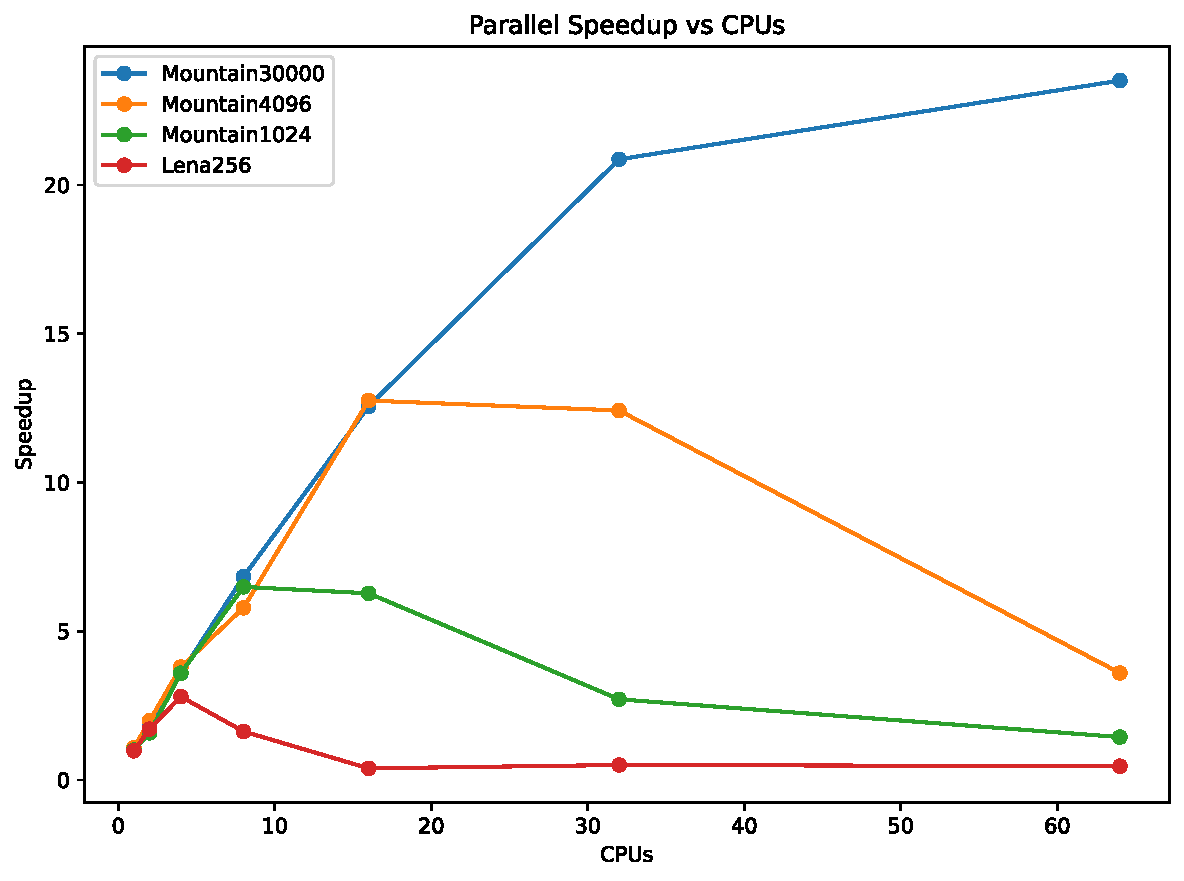
\includegraphics[width=0.8\linewidth]{./pics/speedupPlot.pdf}
    \caption{Speedup ανα Cores για διαφορετικά μεγέθους προβλήματα}
\end{figure}

Μπορούμε να παρατηρήσουμε ότι για μικρές εικόνες (μικρό μεγέθους πρόβλημα) το speedup αρχίζει να μειώνεται όσο αυξάνονται οι πυρήνες. Αυτό συμβαίνει γιατί οι γραμμές που παίρνει κάθε πυρήνας μειώνονται πολύ, σε βαθμό που ο έξτρα κώδικας που χρειάζεται ο παράλληλος αλγόριθμος για να κληθούν οι διαφορετικοί πυρήνες και να συγχρονιστούν προκαλούν την μείωση της απόδοσης του. Όσο μεγαλώνουν οι εικόνες (μεγαλώνει το μέγεθος του προβλήματος) ο κάθε πυρήνας έχει περισσότερες γραμμές να επεξεργαστεί οπότε η απόδοση αρχίζει να μειώνεται για μεγαλύτερο πλήθος πυρήνων. Για την εικόνα \verb|mountain30000|, που έχει πάρα πολλές γραμμές, δεν μπορούμε να δούμε με τους 64 πυρήνες μείωση του speedup.\\

Σημείωση, ότι τα πειραματικά αποτελέσματα πάρθηκαν ενώ έτρεχε στον pxeon2 ένα άλλο πρόγραμμα που χρησιμοποιούσε σχεδόν 90\% του επεξεργαστή, οπότε τα αποτελέσματα θα μπορούσαν να είναι και καλύτερα.



\section[Παράλληλη Υλοποίηση του Αλγόριθμου σε Κάρτα Γραφικών (Cuda)]{Παράλληλη Υλοποίηση του Αλγόριθμου σε Κάρτα\\[-0.8em] Γραφικών (Cuda)}

Για την παραλληλοποιήση σε cuda απλά μετέτρεψα την παράλληλη συνάρτηση που κάνει τα περάσματα της εικόνας από των κώδικα openmp για παραλληλοποιήση σε επεξεργαστή, στον αντίστοιχο κώδικα cuda. Οπότε κατέληξα στο παρακάτω kernel function που τρέχει στην GPU.

\begin{minted}[breaklines, breaksymbolright={}, breaksymbolleft={}, bgcolor=paraiso-light]{c}
 __global__ void crimmins_pass_kernel(uint8_t *out, const uint8_t *in,
                  int width, int height, int dx, int dy, int is_light)
 {
     int x = blockIdx.x * blockDim.x + threadIdx.x + 1;
     int y = blockIdx.y * blockDim.y + threadIdx.y + 1;

     if (x >= width - 1 || y >= height - 1) return;

     uint8_t a = in[(y - dy) * width + (x - dx)];
     uint8_t b = in[y * width + x];
     uint8_t c = in[(y + dy) * width + (x + dx)];

     b = is_light ? light_pass_logic_dev(a, b, c) :
                    dark_pass_logic_dev(a, b, c);

     out[y * width + x] = b;
 }
\end{minted}

Όπως και με της προηγούμενές υλοποιήσεις της συνάρτησης τα ορίσματα παραμένουν ίδια. Αρχικά υπολογίζουμε τις συντεταγμένες x και y που θα πάρει το κάθε νήμα που θα τρέξει το kernel με βάση τα blockId και τα threadId τους και προσθέτουμε 1 έτσι ώστε να ξεκινήσουν από το (1, 1) της εικόνας και όχι από το (0, 0). Έπειτα, ελέγχουμε αν δεν ξεπερνάει τα όρια της εικόνας και κάνουμε τον υπολογισμό των pixel με τον ίδιο τρόπο. Πάλι η επιλογή των ζευγαριών που θα κάνει το κάθε πέρασμα και το αν θα κάνει διόρθωση των σκοτεινών ή φωτεινών pixel επιλέγεται παραμετροποιημένα από τα ορίσματα της συνάρτησης. Οι συναρτήσεις της λογικής διόρθωσης είναι οι ίδιες απλά έβαλα στο όρισμα των συναρτήσεων \verb|__device__| για να μπορώ να τις καλέσω από την GPU.

Για να καλέσω το kernel έχω την ακόλουθη συνάρτηση. Αρχικοποιεί τα events για την μέτρηση χρόνου, φτιάχνει τα δύο buffers που θα έχουν την εικόνα στην μνήμη του GPU και την αντιγράφει εκεί. Έπειτα, ορίζουμε το μέγεθος του grid και των block, δηλαδή πόσα block θα χρησιμοποιήσουμε με πόσα threads το καθένα. Επέλεξα να έχω blocks με 32x32 threads (1024 threads). Τα blocks που χρειαζόμαστε υπολογίζονται με βάση τις διαστάσεις της εικόνας.
Μετά, καλώ το kernel 8 φορές για τα 8 περάσματα τις εικόνας και επαναλαμβάνω για όσες επαναλήψεις έχω. Τέλος, μεταφέρω το αποτέλεσμα στον host, κάνω free τις μεταβλητές και μετράω τον χρόνο που χρειάστηκε.

\begin{minted}[breaklines, breaksymbolright={}, breaksymbolleft={}, bgcolor=paraiso-light]{c}
 float crimmings_speckle_removal_filter_cuda(uint8_t *h_image,
             uint32_t width, uint32_t height, uint8_t iterations)
 {
     size_t numPixels = (size_t)(width * height);
     size_t bufBytes = numPixels * sizeof(uint8_t);

     cudaEvent_t start, stop;
     cudaEventCreate(&start);
     cudaEventCreate(&stop);
     cudaEventRecord(start, 0);

     uint8_t *d_in = NULL;
     uint8_t *d_out = NULL;
     CHECK_CUDA(cudaMalloc((void **)&d_in, bufBytes));
     CHECK_CUDA(cudaMalloc((void **)&d_out, bufBytes));

     CHECK_CUDA(cudaMemcpy(d_in, h_image, bufBytes, cudaMemcpyHostToDevice));
     CHECK_CUDA(cudaMemcpy(d_out, h_image, bufBytes, cudaMemcpyDeviceToDevice));

     dim3 block = {32, 32, 1};
     dim3 grid = {
         (uint32_t)((width + block.x - 3) / block.x),
         (uint32_t)((height + block.y - 3) / block.y),
         1
     };
     for (int iter = 0; iter < iterations; iter++) {
         for (int p = 0; p < 8; p++) {
             int is_light = (passes[p].pass_logic_func == light_pass_logic);

             crimmins_pass_kernel<<<grid, block>>>(
             d_out, d_in, width, height, passes[p].dx, passes[p].dy, is_light);

             SWAP(d_out, d_in);
         }
     }
     CHECK_CUDA(cudaMemcpy(h_image, d_out, bufBytes, cudaMemcpyDeviceToHost));

     cudaEventRecord(stop, 0);
     cudaEventSynchronize(stop);
     float time = 0;
     cudaEventElapsedTime(&time, start, stop);

     cudaEventDestroy(start);
     cudaEventDestroy(stop);

     cudaFree(d_buf1);
     cudaFree(d_buf2);
     return time * 1e-3f; // convert to sec
 }
\end{minted}

\section{Πειραματικά αποτελέσματα CUDA}

\begin{table}[H]
\caption*{\large 1 Iteration}
    \centering
    \begin{subtable}[t]{0.48\textwidth}
        \centering
        \pgfplotstabletypeset[
        col sep=tab,
        header=true,
        columns={cuda,{mri512.raw/1 (serial)},{mri512.raw/1 (parallel)},{mri512.raw/1 (speedup)}},
        columns/{mri512.raw/1 (serial)}/.style={column name=Ts,fixed,precision=4},
        columns/{mri512.raw/1 (parallel)}/.style={column name=Tp,fixed,precision=4},
        columns/{mri512.raw/1 (speedup)}/.style={column name=Sp,fixed,precision=3},
        column type=c,
        every first column/.style={column type=|c},
        column type/.add={|}{|},
        every head row/.style={
            before row=\hline,
            after row=\hline
        },
        every row/.style={
            before row=\hline
        },
        every last row/.style={
            after row=\hline
        }
        ]{./data/cudaCom.csv}
        \caption{mri512.raw with 1 iteration}
    \end{subtable}%
    \hfill
    \begin{subtable}[t]{0.48\textwidth}
        \centering
        \pgfplotstabletypeset[
        col sep=tab,
        header=true,
        columns={cuda,{mountain1024.raw/1 (serial)},{mountain1024.raw/1 (parallel)},{mountain1024.raw/1 (speedup)}},
        columns/threads/.style={column name=CPUs},
        columns/{mountain1024.raw/1 (serial)}/.style={column name=Ts,fixed,precision=4},
        columns/{mountain1024.raw/1 (parallel)}/.style={column name=Tp,fixed,precision=4},
        columns/{mountain1024.raw/1 (speedup)}/.style={column name=Sp,fixed,precision=2},
        column type=c,
        every first column/.style={column type=|c},
        column type/.add={|}{|},
        every head row/.style={
            before row=\hline,
            after row=\hline
        },
        every row/.style={
            before row=\hline
        },
        every last row/.style={
            after row=\hline
        }
        ]{./data/cudaCom.csv}
        \caption{mountain1024.raw with 1 iteration}
    \end{subtable}

    \vspace{8pt}

    \begin{subtable}[t]{0.48\textwidth}
        \centering
        \pgfplotstabletypeset[
        col sep=tab,
        header=true,
        columns={cuda,{mountain4096.raw/1 (serial)},{mountain4096.raw/1 (parallel)},{mountain4096.raw/1 (speedup)}},
        columns/{mountain4096.raw/1 (serial)}/.style={column name=Ts,fixed,precision=4},
        columns/{mountain4096.raw/1 (parallel)}/.style={column name=Tp,fixed,precision=4},
        columns/{mountain4096.raw/1 (speedup)}/.style={column name=Sp,fixed,precision=2},
        column type=c,
        every first column/.style={column type=|c},
        column type/.add={|}{|},
        every head row/.style={
            before row=\hline,
            after row=\hline
        },
        every row/.style={
            before row=\hline
        },
        every last row/.style={
            after row=\hline
        }
        ]{./data/cudaCom.csv}
        \caption{mountain4096.raw with 1 iteration}
    \end{subtable}%
    \hfill
    \begin{subtable}[t]{0.48\textwidth}
        \centering
        \pgfplotstabletypeset[
        col sep=tab,
        header=true,
        columns={cuda,{mountain30000.raw/1 (serial)},{mountain30000.raw/1 (parallel)},{mountain30000.raw/1 (speedup)}},
        columns/{mountain30000.raw/1 (serial)}/.style={column name=Ts,fixed,precision=4},
        columns/{mountain30000.raw/1 (parallel)}/.style={column name=Tp,fixed,precision=4},
        columns/{mountain30000.raw/1 (speedup)}/.style={column name=Sp,fixed,precision=2},
        column type=c,
        every first column/.style={column type=|c},
        column type/.add={|}{|},
        every head row/.style={
            before row=\hline,
            after row=\hline
        },
        every row/.style={
            before row=\hline
        },
        every last row/.style={
            after row=\hline
        }
        ]{./data/cudaCom.csv}
        \caption{mountain30000.raw with 1 iteration}
    \end{subtable}
\end{table}

\begin{table}[H]
\caption*{\large 4 Iterations}
    \centering
    \begin{subtable}[t]{0.48\textwidth}
        \centering
        \pgfplotstabletypeset[
        col sep=tab,
        header=true,
        columns={cuda,{mri512.raw/4 (serial)},{mri512.raw/4 (parallel)},{mri512.raw/4 (speedup)}},
        columns/{mri512.raw/4 (serial)}/.style={column name=Ts,fixed,precision=4},
        columns/{mri512.raw/4 (parallel)}/.style={column name=Tp,fixed,precision=4},
        columns/{mri512.raw/4 (speedup)}/.style={column name=Sp,fixed,precision=2},
        column type=c,
        every first column/.style={column type=|c},
        column type/.add={|}{|},
        every head row/.style={
            before row=\hline,
            after row=\hline
        },
        every row/.style={
            before row=\hline
        },
        every last row/.style={
            after row=\hline
        }
        ]{./data/cudaCom.csv}
        \caption{mri512.raw with 4 iteration}
    \end{subtable}%
    \hfill
    \begin{subtable}[t]{0.48\textwidth}
        \centering
        \pgfplotstabletypeset[
        col sep=tab,
        header=true,
        columns={cuda,{mountain1024.raw/4 (serial)},{mountain1024.raw/4 (parallel)},{mountain1024.raw/4 (speedup)}},
        columns/threads/.style={column name=CPUs},
        columns/{mountain1024.raw/4 (serial)}/.style={column name=Ts,fixed,precision=4},
        columns/{mountain1024.raw/4 (parallel)}/.style={column name=Tp,fixed,precision=4},
        columns/{mountain1024.raw/4 (speedup)}/.style={column name=Sp,fixed,precision=2},
        column type=c,
        every first column/.style={column type=|c},
        column type/.add={|}{|},
        every head row/.style={
            before row=\hline,
            after row=\hline
        },
        every row/.style={
            before row=\hline
        },
        every last row/.style={
            after row=\hline
        }
        ]{./data/cudaCom.csv}
        \caption{mountain1024.raw with 4 iteration}
    \end{subtable}

    \vspace{8pt}

    \begin{subtable}[t]{0.48\textwidth}
        \centering
        \pgfplotstabletypeset[
        col sep=tab,
        header=true,
        columns={cuda,{mountain4096.raw/4 (serial)},{mountain4096.raw/4 (parallel)},{mountain4096.raw/4 (speedup)}},
        columns/{mountain4096.raw/4 (serial)}/.style={column name=Ts,fixed,precision=4},
        columns/{mountain4096.raw/4 (parallel)}/.style={column name=Tp,fixed,precision=4},
        columns/{mountain4096.raw/4 (speedup)}/.style={column name=Sp,fixed,precision=2},
        column type=c,
        every first column/.style={column type=|c},
        column type/.add={|}{|},
        every head row/.style={
            before row=\hline,
            after row=\hline
        },
        every row/.style={
            before row=\hline
        },
        every last row/.style={
            after row=\hline
        }
        ]{./data/cudaCom.csv}
        \caption{mountain4096.raw with 4 iteration}
    \end{subtable}%
    \hfill
    \begin{subtable}[t]{0.48\textwidth}
        \centering
        \pgfplotstabletypeset[
        col sep=tab,
        header=true,
        columns={cuda,{mountain30000.raw/4 (serial)},{mountain30000.raw/4 (parallel)},{mountain30000.raw/4 (speedup)}},
        columns/{mountain30000.raw/4 (serial)}/.style={column name=Ts,fixed,precision=4},
        columns/{mountain30000.raw/4 (parallel)}/.style={column name=Tp,fixed,precision=4},
        columns/{mountain30000.raw/4 (speedup)}/.style={column name=Sp,fixed,precision=2},
        column type=c,
        every first column/.style={column type=|c},
        column type/.add={|}{|},
        every head row/.style={
            before row=\hline,
            after row=\hline
        },
        every row/.style={
            before row=\hline
        },
        every last row/.style={
            after row=\hline
        }
        ]{./data/cudaCom.csv}
        \caption{mountain30000.raw with 4 iteration}
    \end{subtable}
\end{table}

\begin{table}[H]
\caption*{\large 10 Iterations}
    \centering
    \begin{subtable}[t]{0.48\textwidth}
        \centering
        \pgfplotstabletypeset[
        col sep=tab,
        header=true,
        columns={cuda,{mri512.raw/10 (serial)},{mri512.raw/10 (parallel)},{mri512.raw/10 (speedup)}},
        columns/{mri512.raw/10 (serial)}/.style={column name=Ts,fixed,precision=4},
        columns/{mri512.raw/10 (parallel)}/.style={column name=Tp,fixed,precision=4},
        columns/{mri512.raw/10 (speedup)}/.style={column name=Sp,fixed,precision=2},
        column type=c,
        every first column/.style={column type=|c},
        column type/.add={|}{|},
        every head row/.style={
            before row=\hline,
            after row=\hline
        },
        every row/.style={
            before row=\hline
        },
        every last row/.style={
            after row=\hline
        }
        ]{./data/cudaCom.csv}
        \caption{mri512.raw with 10 iteration}
    \end{subtable}%
    \hfill
    \begin{subtable}[t]{0.48\textwidth}
        \centering
        \pgfplotstabletypeset[
        col sep=tab,
        header=true,
        columns={cuda,{mountain1024.raw/10 (serial)},{mountain1024.raw/10 (parallel)},{mountain1024.raw/10 (speedup)}},
        columns/threads/.style={column name=CPUs},
        columns/{mountain1024.raw/10 (serial)}/.style={column name=Ts,fixed,precision=4},
        columns/{mountain1024.raw/10 (parallel)}/.style={column name=Tp,fixed,precision=4},
        columns/{mountain1024.raw/10 (speedup)}/.style={column name=Sp,fixed,precision=2},
        column type=c,
        every first column/.style={column type=|c},
        column type/.add={|}{|},
        every head row/.style={
            before row=\hline,
            after row=\hline
        },
        every row/.style={
            before row=\hline
        },
        every last row/.style={
            after row=\hline
        }
        ]{./data/cudaCom.csv}
        \caption{mountain1024.raw with 10 iteration}
    \end{subtable}

    \vspace{8pt}

    \begin{subtable}[t]{0.48\textwidth}
        \centering
        \pgfplotstabletypeset[
        col sep=tab,
        header=true,
        columns={cuda,{mountain4096.raw/10 (serial)},{mountain4096.raw/10 (parallel)},{mountain4096.raw/10 (speedup)}},
        columns/{mountain4096.raw/10 (serial)}/.style={column name=Ts,fixed,precision=4},
        columns/{mountain4096.raw/10 (parallel)}/.style={column name=Tp,fixed,precision=4},
        columns/{mountain4096.raw/10 (speedup)}/.style={column name=Sp,fixed,precision=2},
        column type=c,
        every first column/.style={column type=|c},
        column type/.add={|}{|},
        every head row/.style={
            before row=\hline,
            after row=\hline
        },
        every row/.style={
            before row=\hline
        },
        every last row/.style={
            after row=\hline
        }
        ]{./data/cudaCom.csv}
        \caption{mountain4096.raw with 10 iteration}
    \end{subtable}%
    \hfill
    \begin{subtable}[t]{0.48\textwidth}
        \centering
        \pgfplotstabletypeset[
        col sep=tab,
        header=true,
        columns={cuda,{mountain30000.raw/10 (serial)},{mountain30000.raw/10 (parallel)},{mountain30000.raw/10 (speedup)}},
        columns/{mountain30000.raw/10 (serial)}/.style={column name=Ts,fixed,precision=4},
        columns/{mountain30000.raw/10 (parallel)}/.style={column name=Tp,fixed,precision=4},
        columns/{mountain30000.raw/10 (speedup)}/.style={column name=Sp,fixed,precision=2},
        column type=c,
        every first column/.style={column type=|c},
        column type/.add={|}{|},
        every head row/.style={
            before row=\hline,
            after row=\hline
        },
        every row/.style={
            before row=\hline
        },
        every last row/.style={
            after row=\hline
        }
        ]{./data/cudaCom.csv}
        \caption{mountain30000.raw with 10 iteration}
    \end{subtable}
\end{table}

Παρατηρούμε, ότι για μικρές εικόνες (μικρού μεγέθους πρόβλημα) ο χρόνος που χρειάζεται για να τρέξει στην GPU είναι μεγαλύτερος από τον σειριακό. Αυτό συμβαίνει γιατί ο χρόνος που χρειάζεται για να μεταφέρει τα δεδομένα των εικόνων από την RAM στην VRAM είναι μεγαλύτερος από ότι να τρέξει ο αλγόριθμος σειριακά. Για μεγαλύτερες εικόνες βλέπουμε να αυξάνει η επιτάχυνση κατά πολύ. Σημαντικό, εδώ είναι να πούμε ότι οι χρόνοι που χρειάζεται για να τρέξει ο αλγόριθμος στην GPU παραμένει σχετικά σταθερός γιατί το ένα πέρασμα της εικόνας γίνεται παράλληλα για όλα τα pixel όσο η εικόνα μπορεί να χωρέσει ολόκληρη στα threads της GPU.

\section{Σύγκριση των υλοποιήσεων}

\begin{figure}[H]
    \centering
    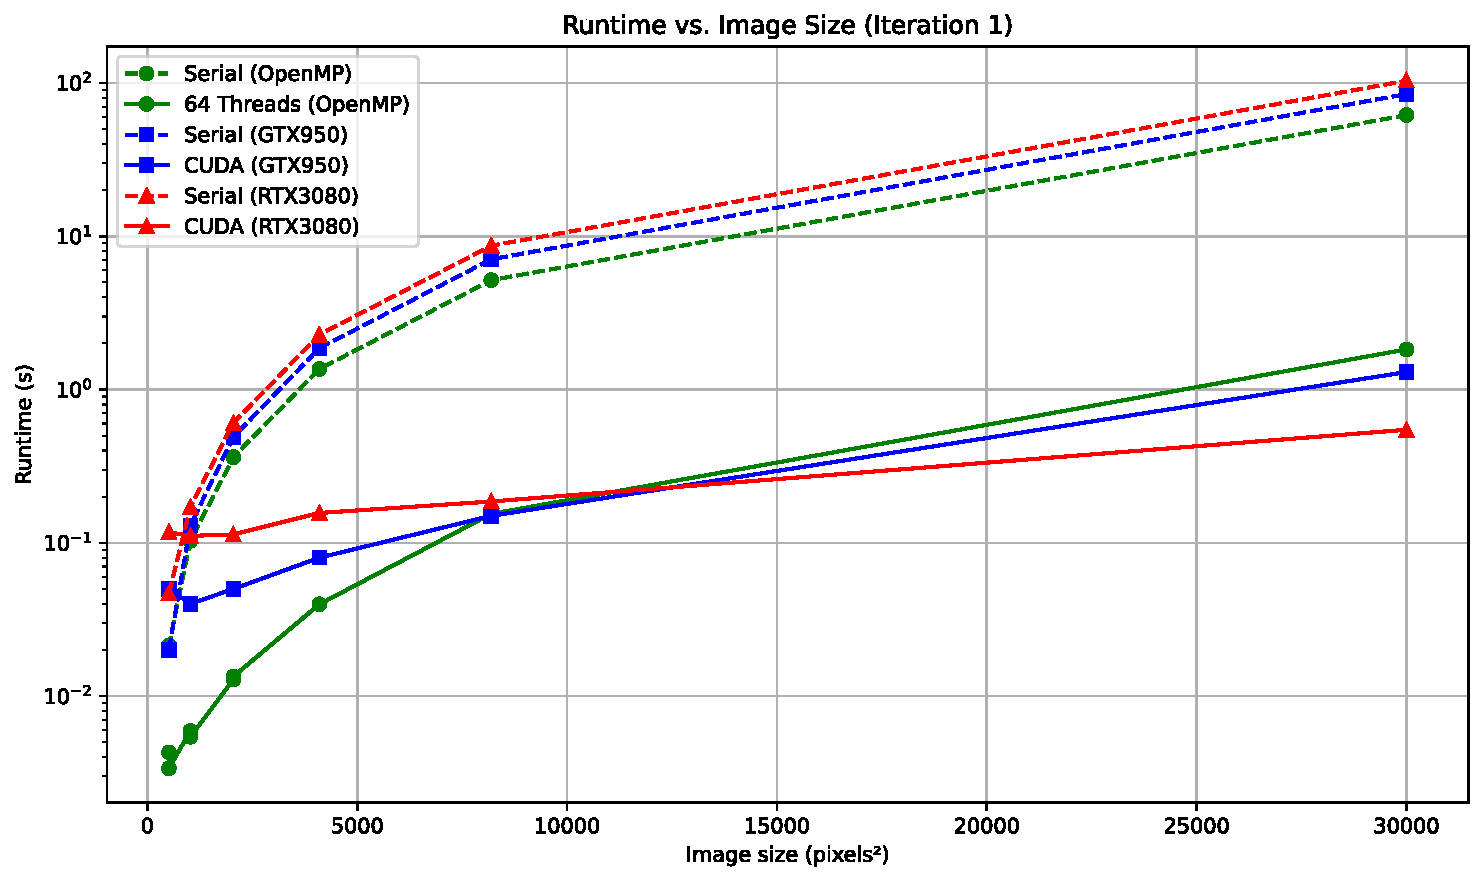
\includegraphics[width=\linewidth]{./pics/runtimeCurves_1.pdf}
    \caption{Χρόνος εκτέλεσης αλγορίθμου προς μέγεθος προβλήματος για μία επανάληψη}
\end{figure}

\begin{figure}[H]
    \centering
    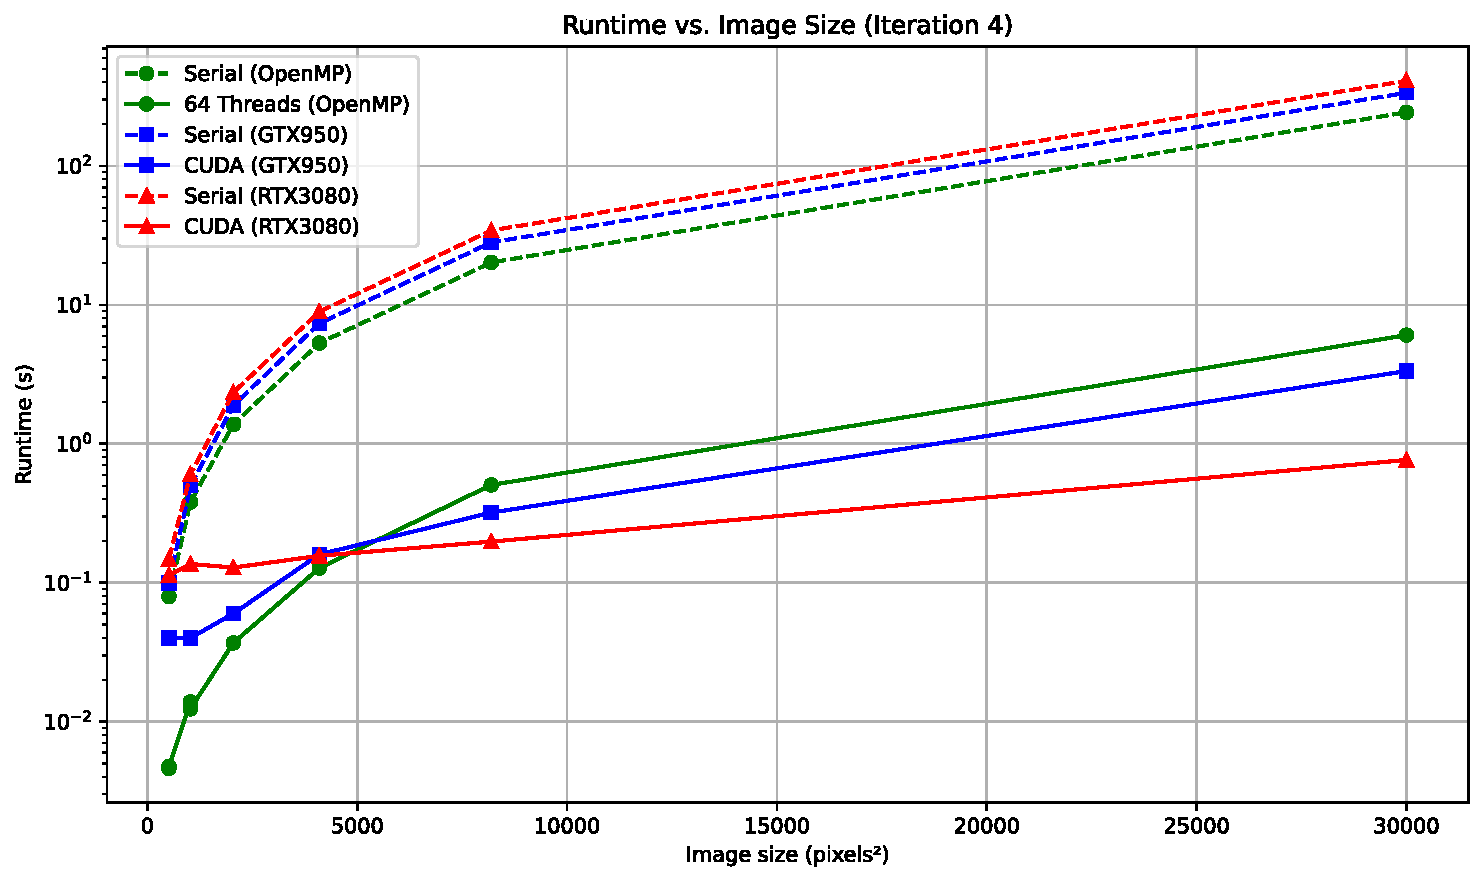
\includegraphics[width=\linewidth]{./pics/runtimeCurves_4.pdf}
    \caption{Χρόνος εκτέλεσης αλγορίθμου προς μέγεθος προβλήματος για τέσσερις επανάληψη}
\end{figure}

\begin{figure}[H]
    \centering
    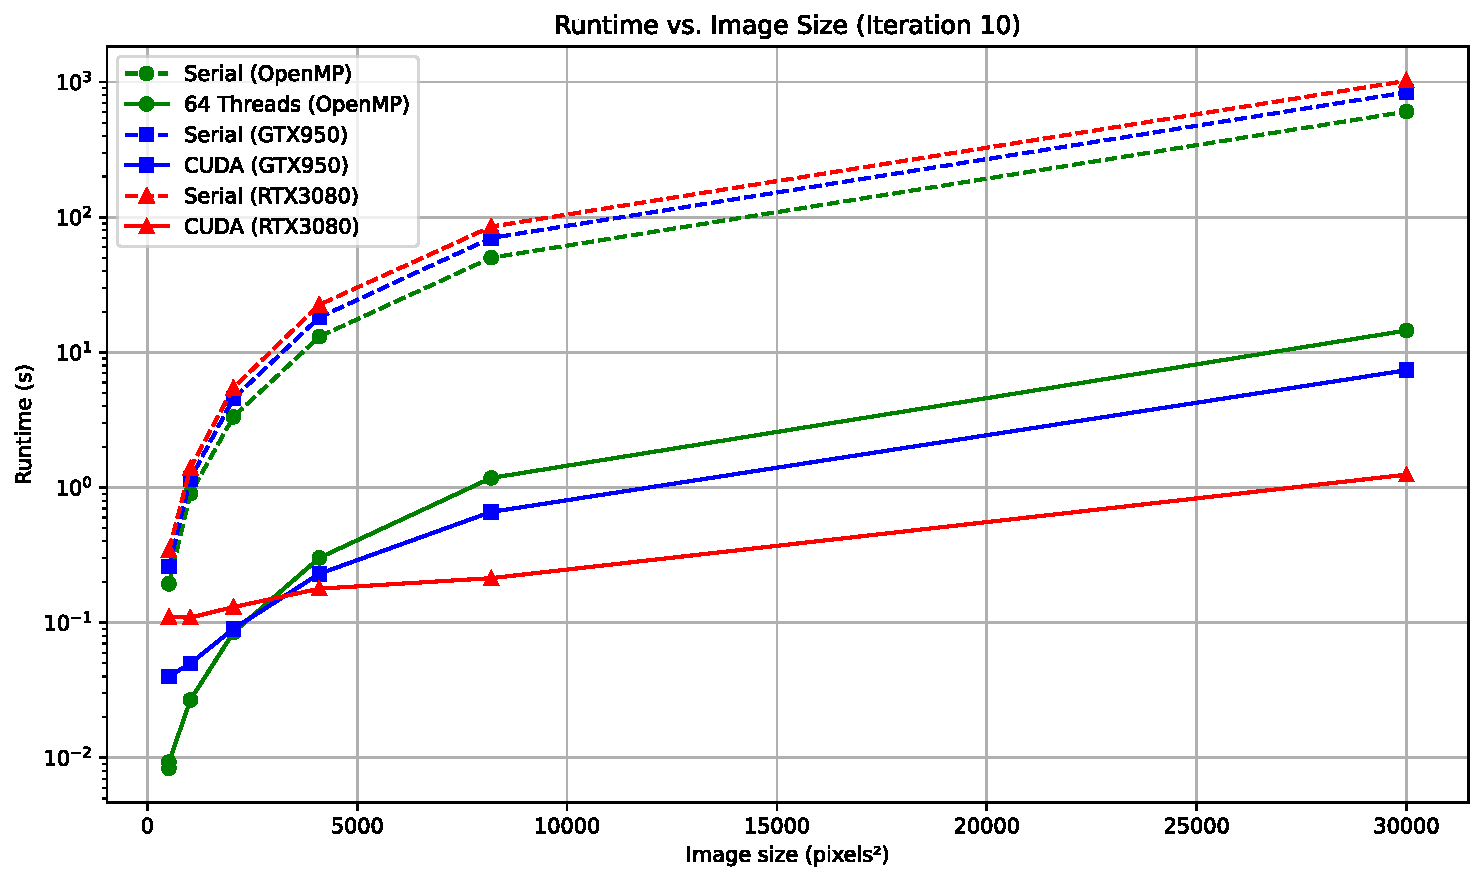
\includegraphics[width=\linewidth]{./pics/runtimeCurves_10.pdf}
    \caption{Χρόνος εκτέλεσης αλγορίθμου προς μέγεθος προβλήματος για δέκα επανάληψη}
\end{figure}

Αρχικά, βλέπουμε ότι οι χρόνοι του σειριακού αλγόριθμου αυξάνεται εκθετικά όσο αυξάνεται το μέγεθος της εικόνας. Ο χρόνος των παράλληλων αλγορίθμων στην GPU παραμένουν σχετικά σταθεροί.

\begin{figure}[H]
    \centering
    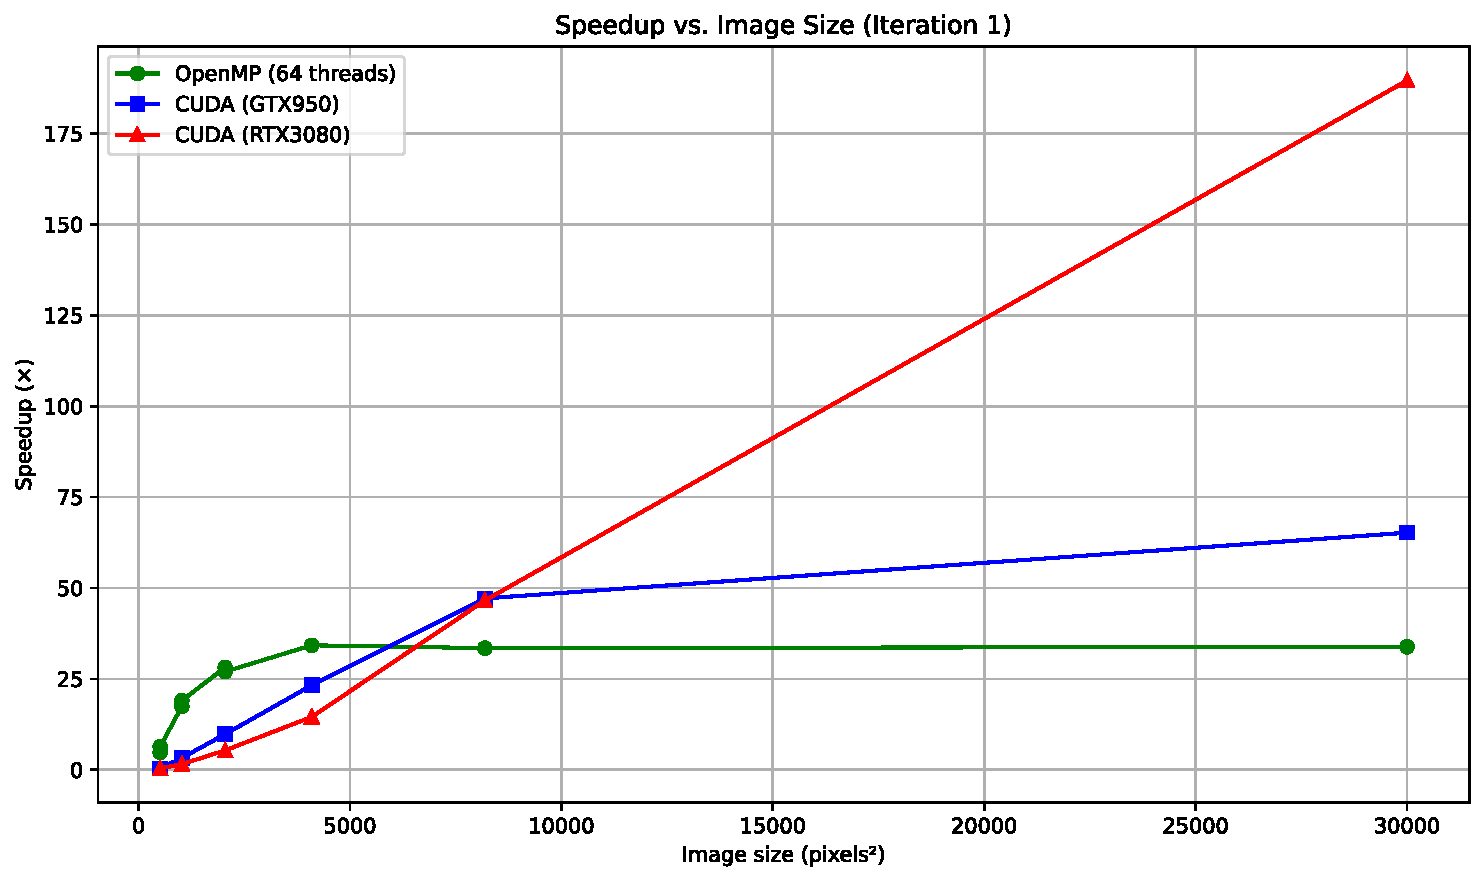
\includegraphics[width=\linewidth]{./pics/speedupCurves_1.pdf}
    \caption{Επιτάχυνση του αλγορίθμου προς το μέγεθος του προβλήματος για μία επανάληψη}
\end{figure}

\begin{figure}[H]
    \centering
    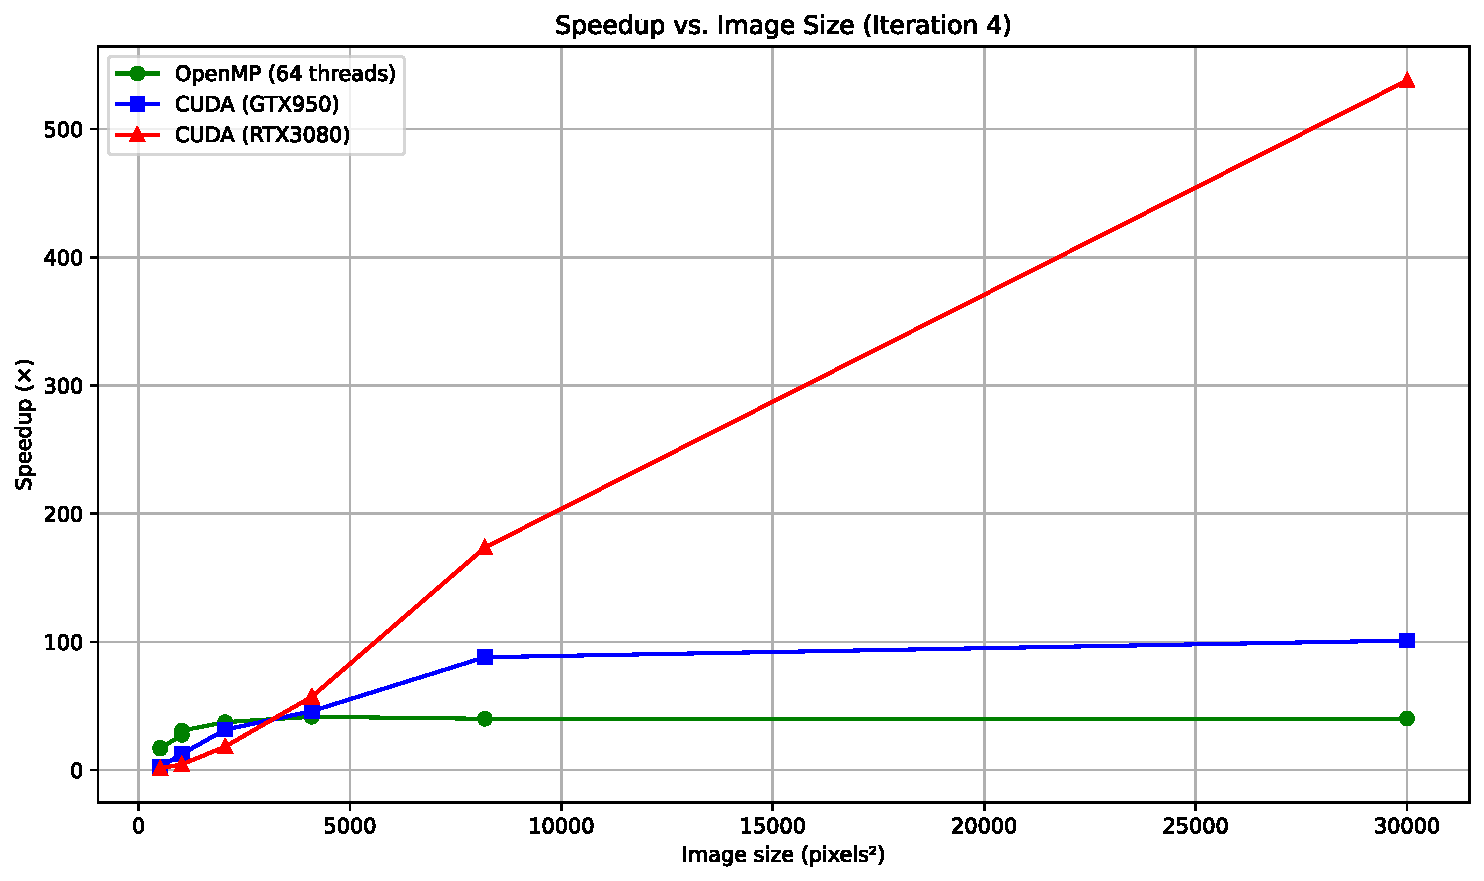
\includegraphics[width=\linewidth]{./pics/speedupCurves_4.pdf}
    \caption{Επιτάχυνση του αλγορίθμου προς το μέγεθος του προβλήματος για τέσσερις επαναλήψεις}
\end{figure}

\begin{figure}[H]
    \centering
    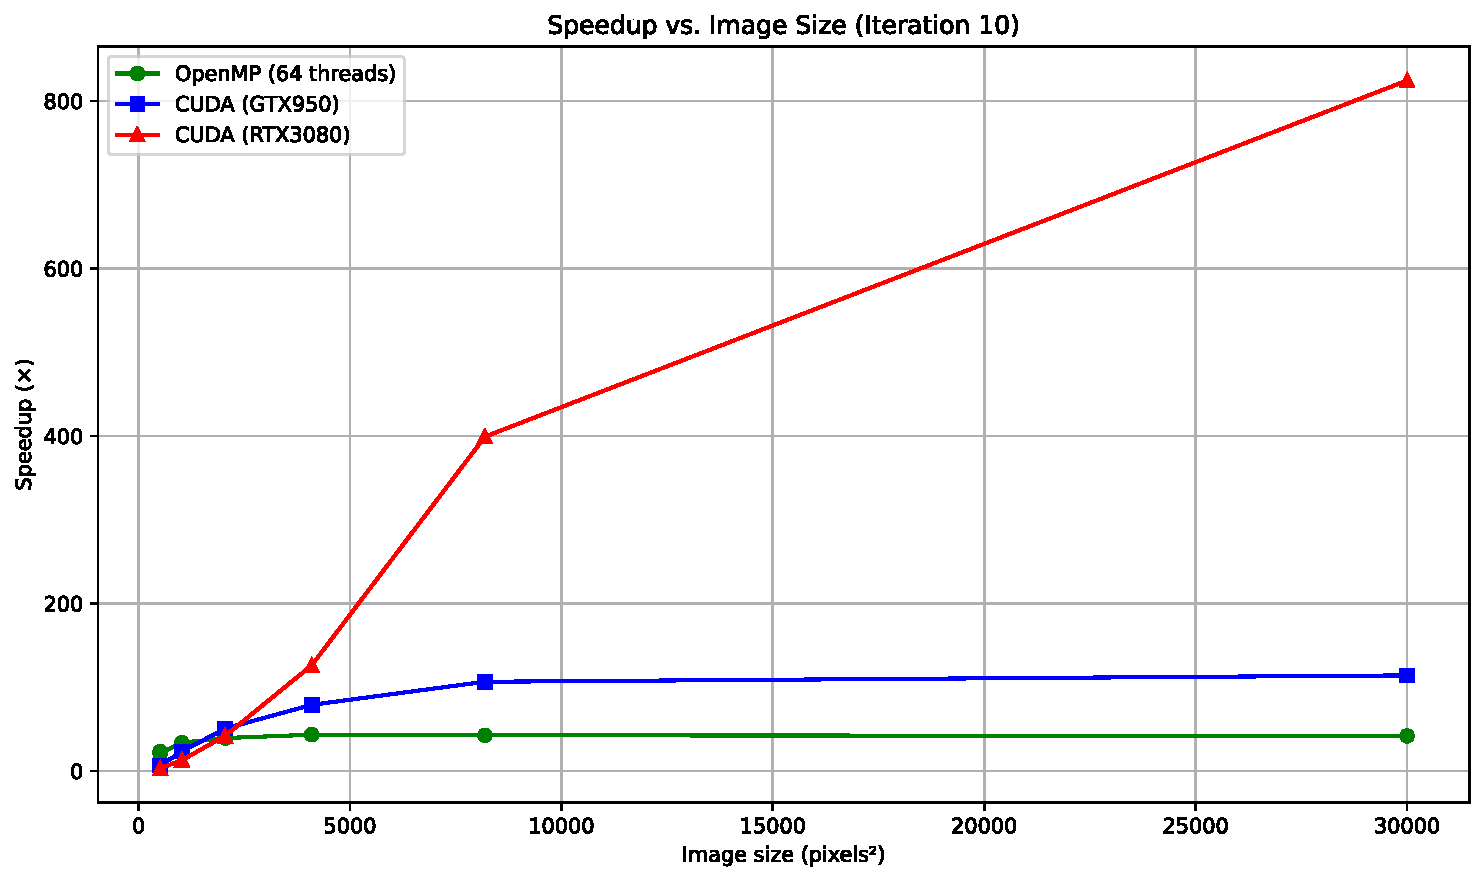
\includegraphics[width=\linewidth]{./pics/speedupCurves_10.pdf}
    \caption{Επιτάχυνση του αλγορίθμου προς το μέγεθος του προβλήματος για δέκα επαναλήψεις}
\end{figure}

Για τον παράλληλο αλγόριθμο στην rtx3080 το speedup συνεχίζει να αυξάνεται γραμμικά οπότε δεν βλέπουμε εδώ τα όρια της πλατφόρμας, όπως βλέπουμε με την gtx950 ή τον 64 πυρήνων CPU.


Για τον παράλληλο αλγόριθμο στην rtx3080 το speedup συνεχίζει να αυξάνεται γραμμικά οπότε δεν βλέπουμε εδώ τα όρια της πλατφόρμας, όπως βλέπουμε με την gtx950 ή τον 64 πυρήνων CPU.

% \newpage
\vspace{1.5em}
\nocite{*}
\printbibliography
\addcontentsline{toc}{section}{Αναφορές}

\end{document}
